\section{Durchführung}
\label{sec:Durchführung}

Der Versuch besteht aus zwei Teilen, die im Folgenden getrennt beschreiben werden.
\subsection{Druckbereich von 30 bis 1000 mbar}
In diesem Teil des Versuchs wird die Dampfdruckkurve von Wasser zwischen 30 bis 1000 mbar bestimmt.
\begin{figure}[H]
    \centering
    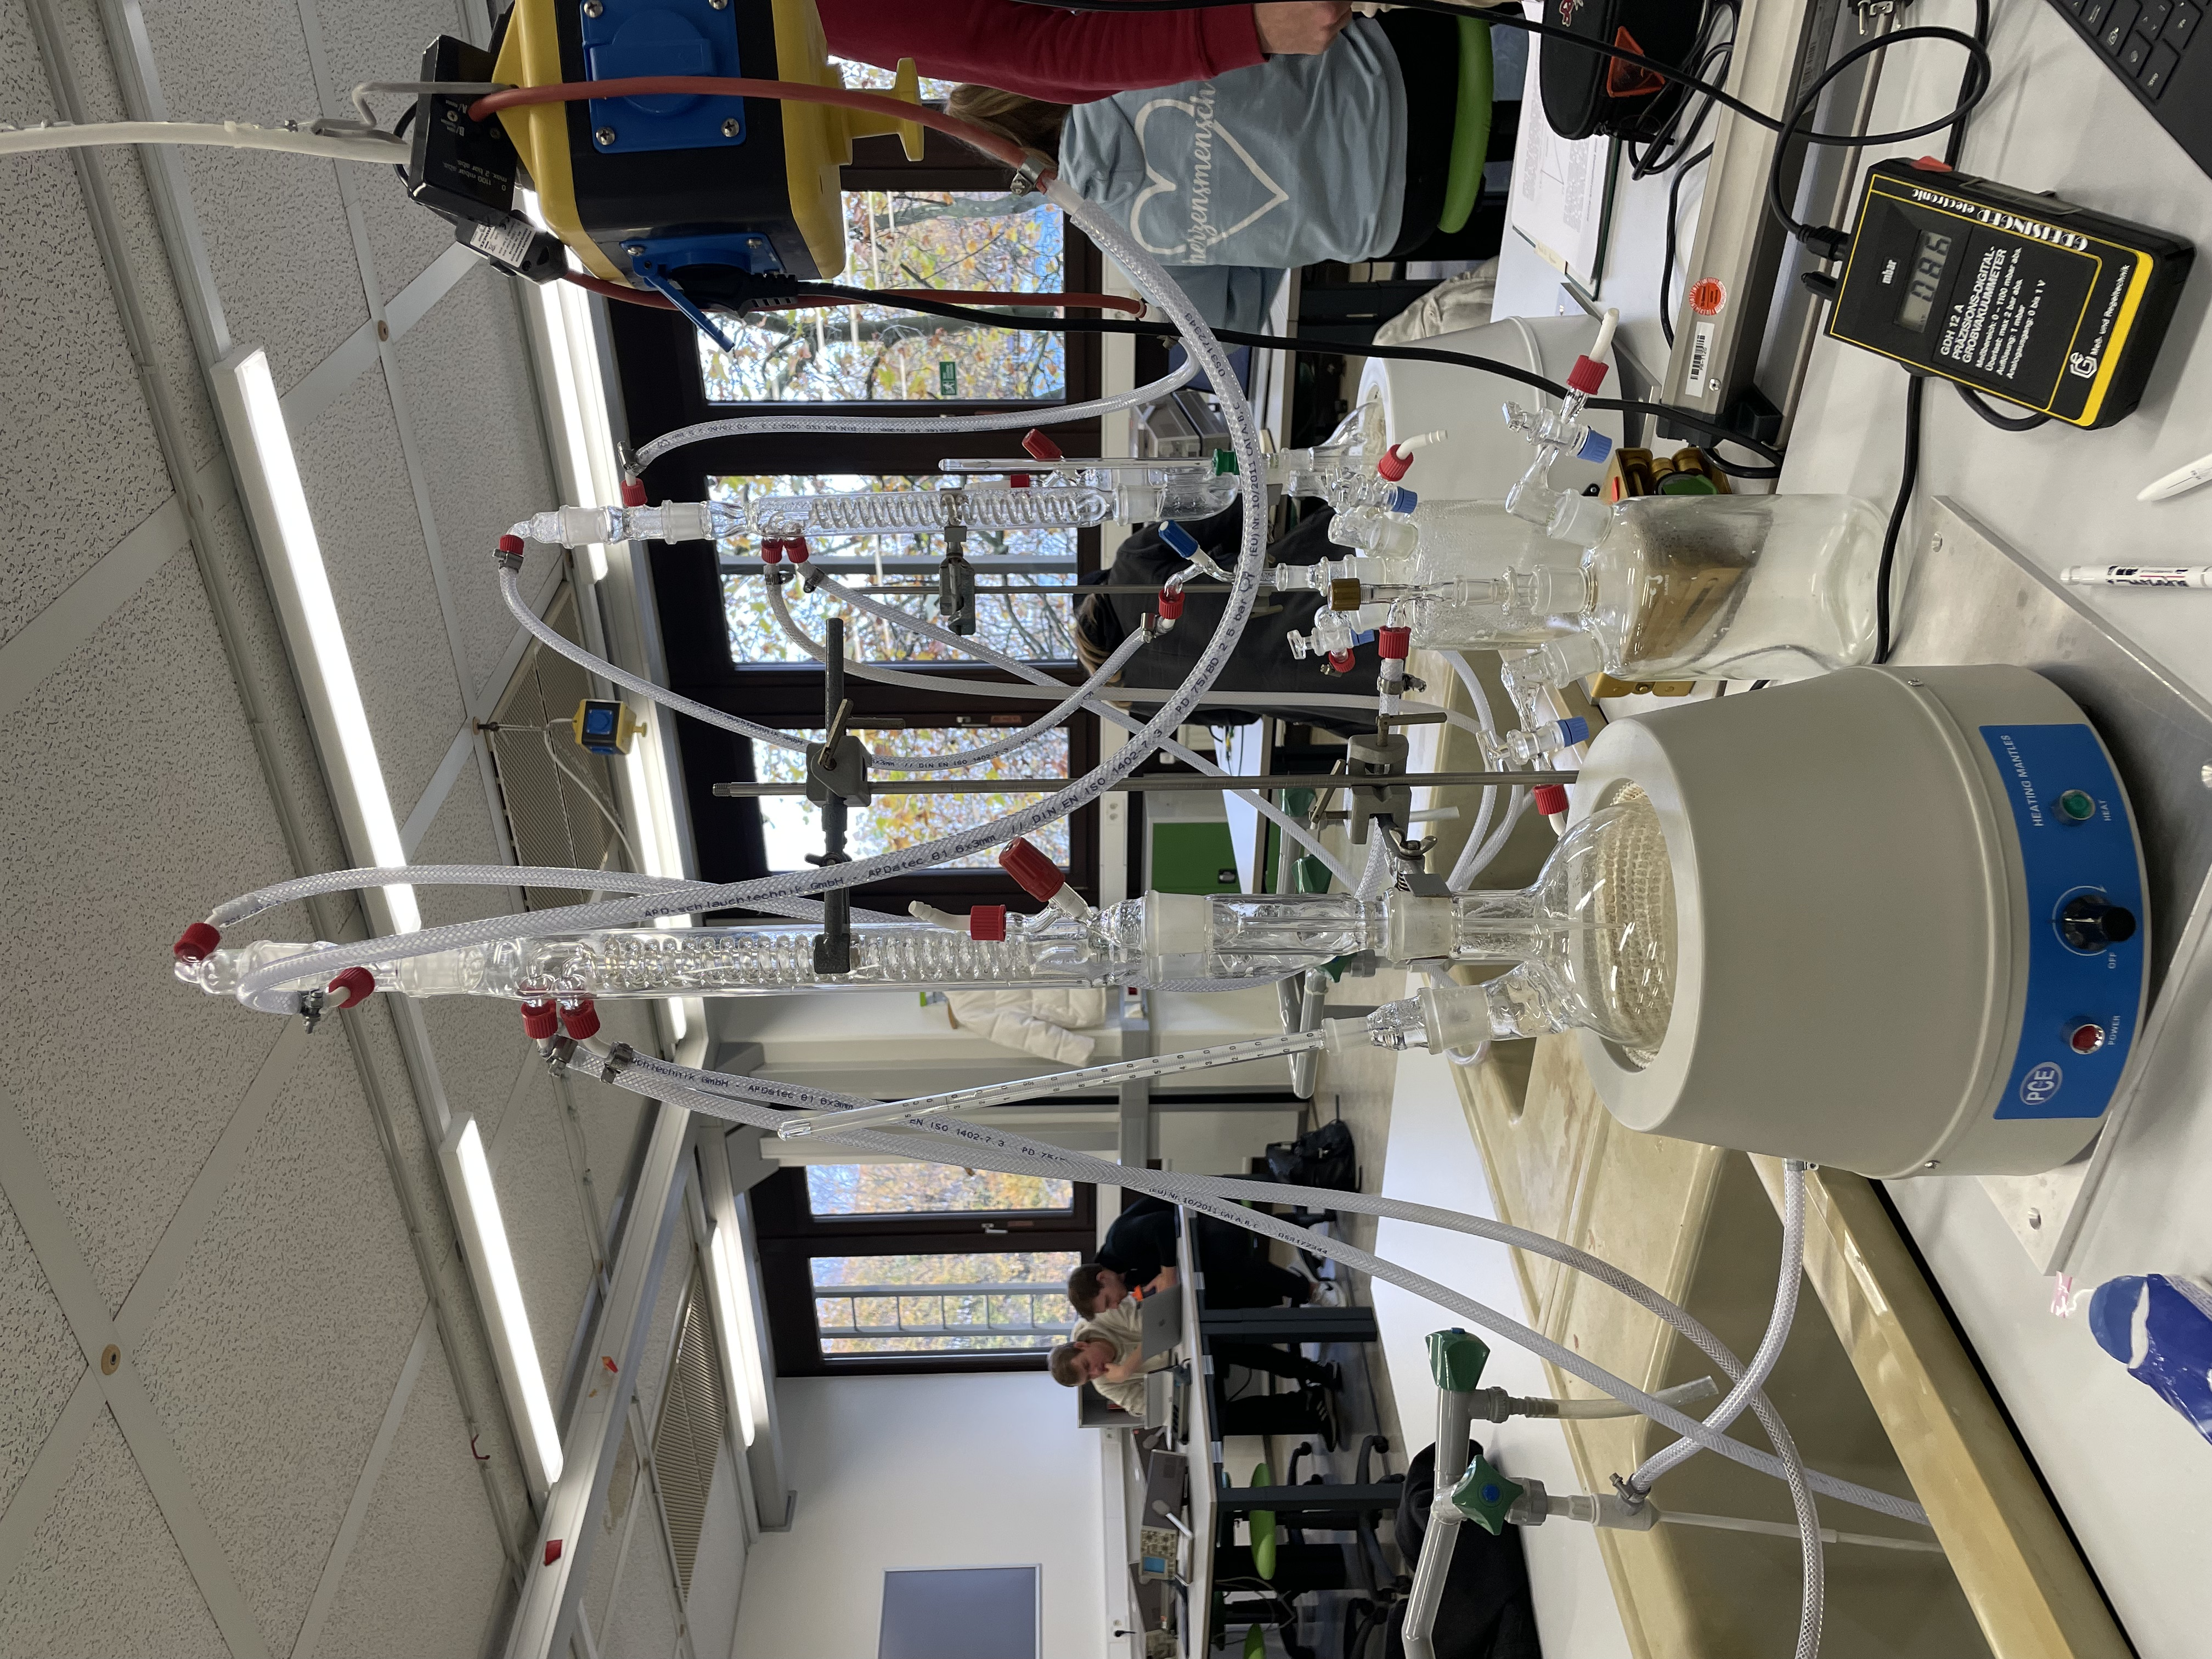
\includegraphics[height=2.7cm, angle=270]{content/Verwendete_Messapparatur.jpeg}
    \caption{Zu sehen ist die verwendete Messapparatur während der Evakuierung.}
    \label{Abb:Messapparatur}
\end{figure}
Eine Wasserstrahlpumpe ist über die Woulffsche Flasche mit dem Rest der Apparatur verbunden.
Diese Flasche lässt sich durch einen Absperrhahn und ein Drosselventiel abriegeln, was im Verlauf des Versuchs noch von größerer Bedeutung sein wird.\\
\begin{figure}[H]
    \centering
    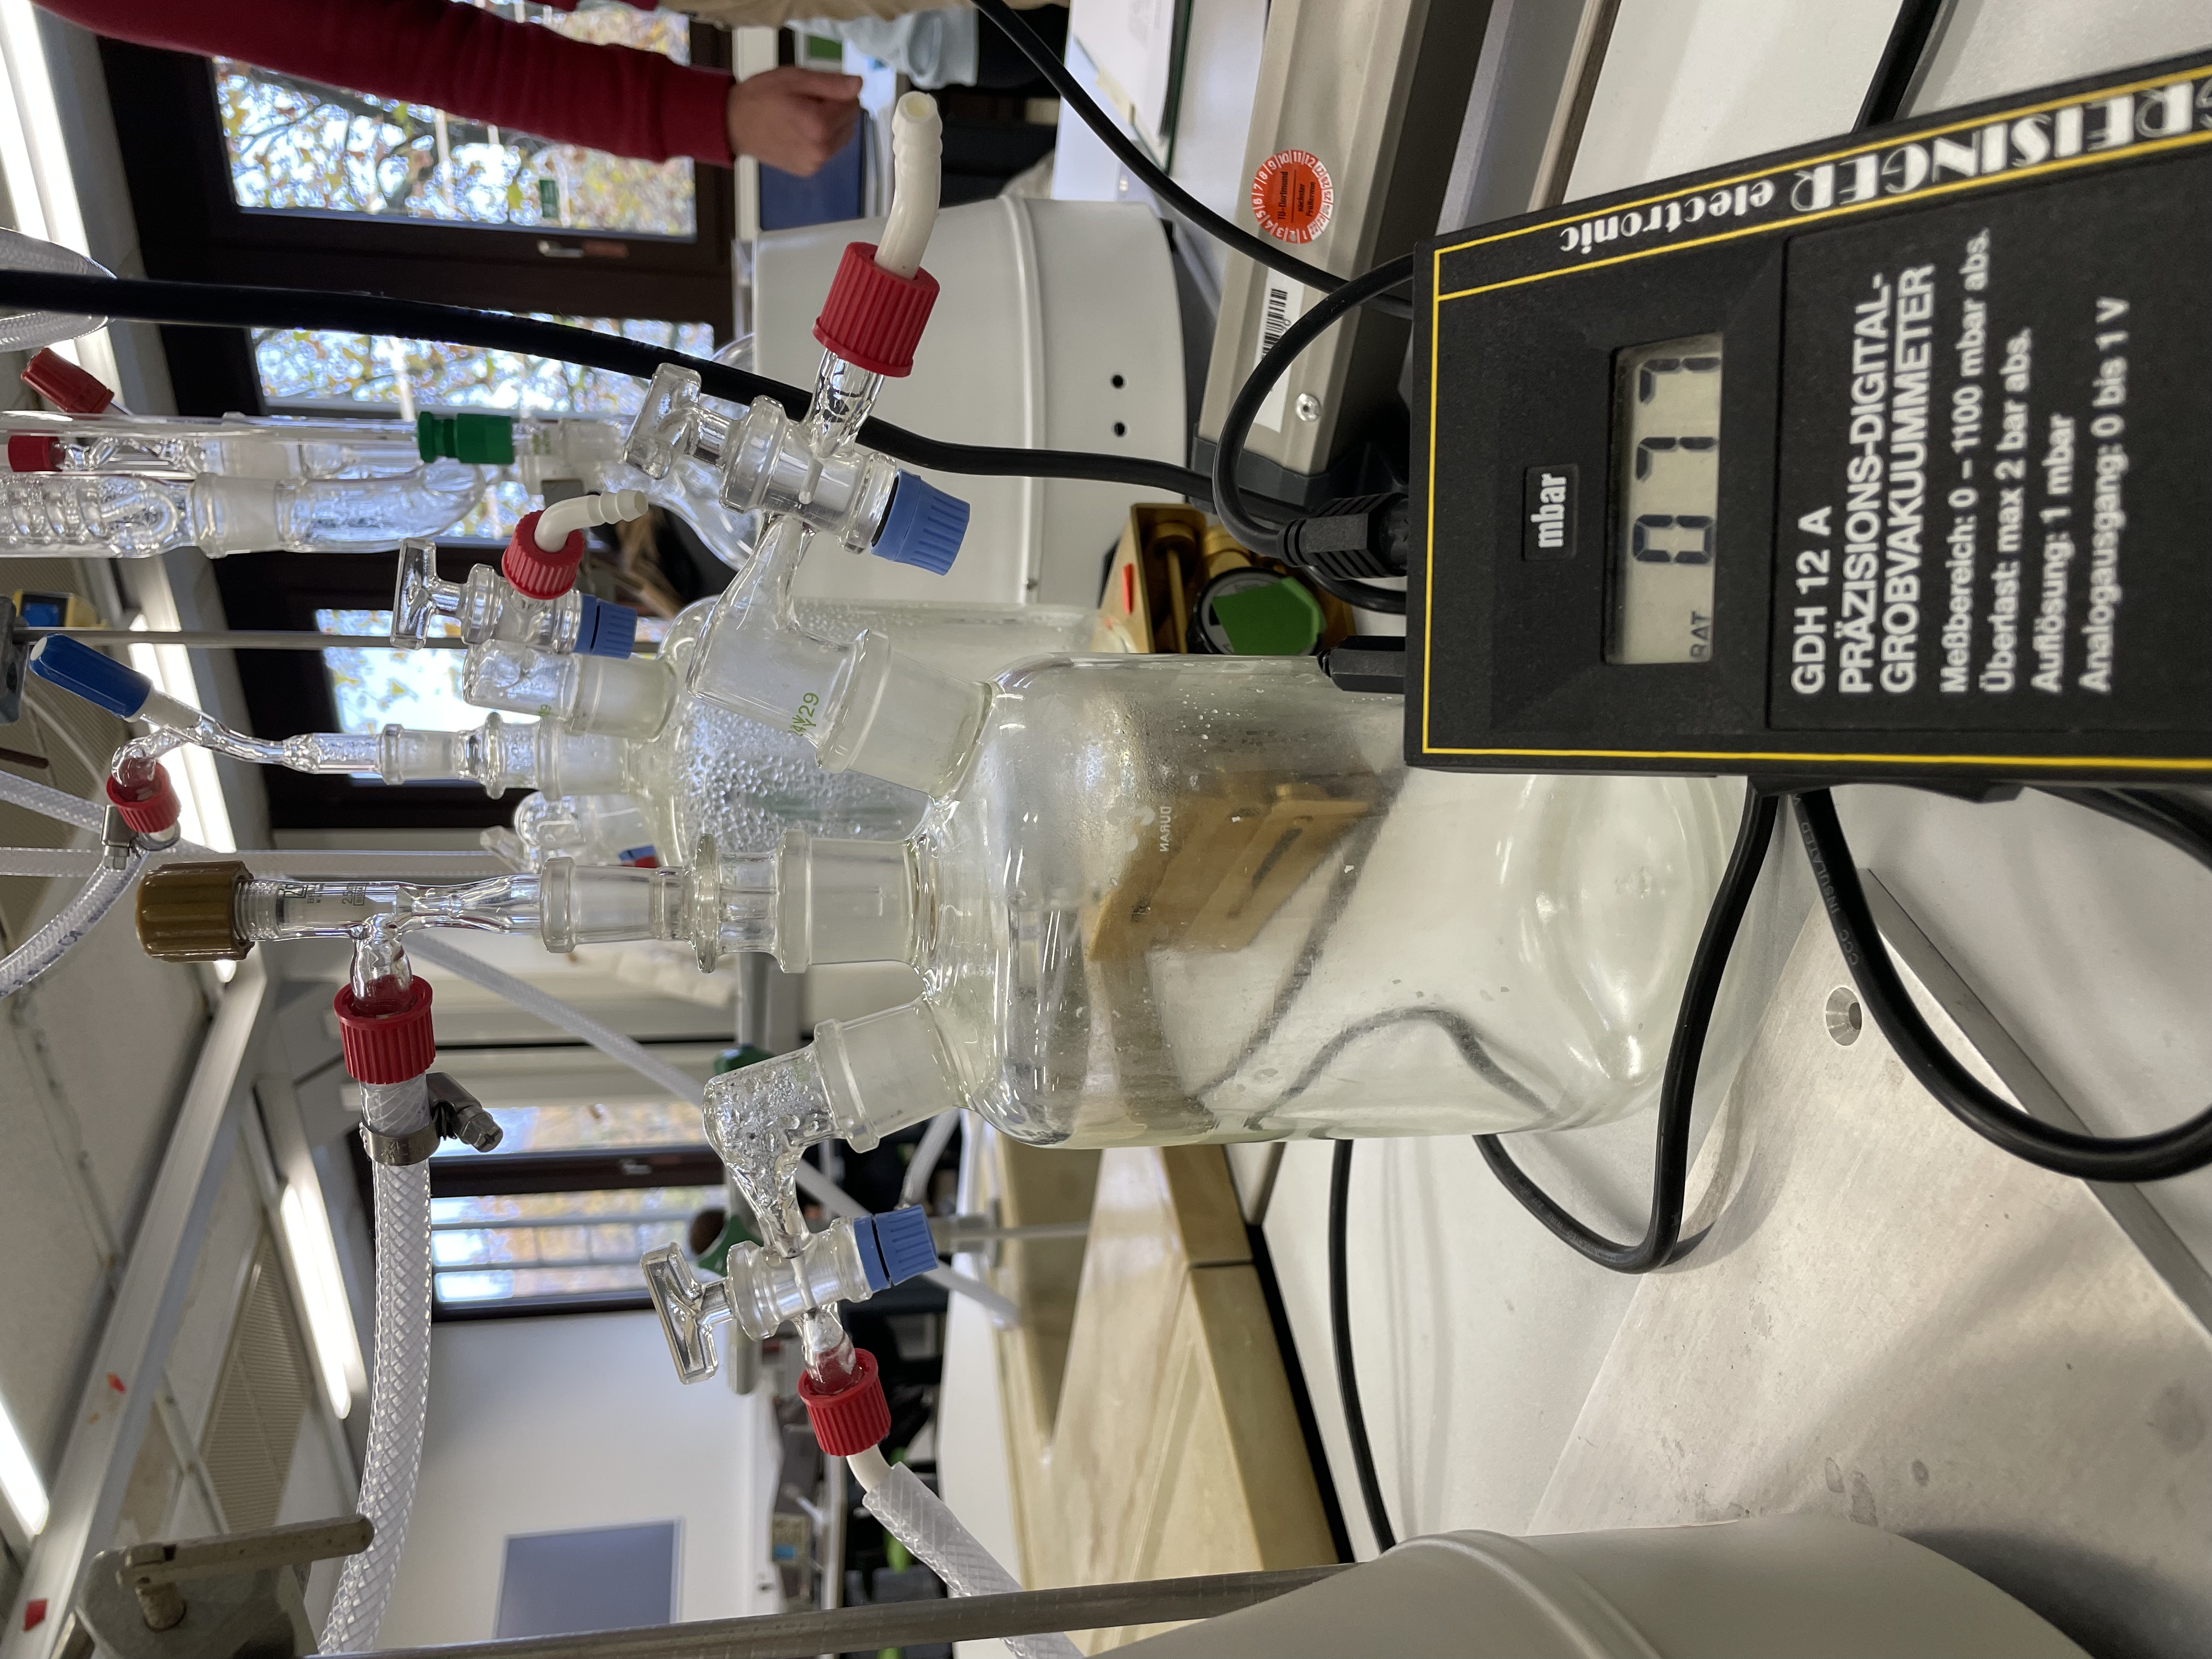
\includegraphics[height=2.7cm, angle=270]{content/Woulffsche_Flasche.jpeg}
    \caption{Die Woulffsche Flasche und das Manometer während der Evakuierung der Apparatur.}
    \label{Abb:Woulffsche_Flasche}
\end{figure}
Ein Manometer ist ebenfalls mit dem Mehrhalskolben verbunden, um kontinuierlich den Dampfdruck im Inneren messen zu können.
Nun folgt die eigentliche Apparatur.
Sie besteht aus einer Heizhaube, die einen Mehrhalskolben erhitzt.
In diesem Kolben befindet sich die zu untersuchende Flüssigkeit.
In diesem Fall handelt es sich um Wasser.
Außerdem befindet sich im Kolben ein Thermometer, so kann die Temperatur zu jeder Zeit abgenommen werden.
Ein Rückflusskühler komplettiert die Messapparatur.
Um zu vermeiden, dass Dämpfe in das Manometer gelangen, kondensiert der Rückflusskühler die aufsteigenden Dämpfe.\\

Zunächst wird die gesamte Apparatur mittels der Wasserstrahlpumpe evakuiert, bis der Druck auf 30 mbar abgesunken ist.
Tiefere Drücke sind aufgrund kleiner Undichtigkeiten und fehlender Stärke der Wasserstrahlpumpe nicht möglich.
Anschließend wird das Drosselventiel geschlossen, woraufhin der Absperrhahn verschlossen wird.
So wird die Apparatur nicht weiter evakuiert und die Messung kann beginnen.

Hierfür wird die Heizhaube angeschaltet und der Druck in Abhängigkeit der Zeit gemessen bis der maximale Messwert des Manometers errreicht ist.
Für dieses Manometer liegt er bei 1100 mbar.

\subsection{Druckbereich von einem bis 15 bar}
Im zweiten Teil des Versuchs wird eine ähnliche Messung für den Druckbereich von 1 bis 15 mbar durchgeführt.
Hierfür muss jedoch eine andere Messapparatur verwendet werden, da die Obige diesem Druck nicht mehr standhalten würde.

Diese Apparatur besteht aus einem hohlen Stahlbolzen, welcher sich über einer Heizapparatur befindet.
In dem Hohlraum befindet sich die Flüssigkeit, in diesem Versuch Wasser.
Die Temperatur dieser Flüssigkeit wird über ein Thermometer angegeben, welches ins Innere des Stahlbolzen ragt.
Anders als in der Anleitung beschrieben wurde hier ein analoges Thermometer genutzt.
Der Druck im Stahlbolzen wird über einen Drucksensor, welcher mit dem Hohlraum verbunden ist, gemessen.

Nun wird die Heizung angeschaltet und die Messung kann beginnen.
Die Temperatur wird mit steigendem Druck gemessen, bis ein Druck von $\SI{15}{\bar}$ erreicht ist.
